\begin{figure}[ht]
\centering
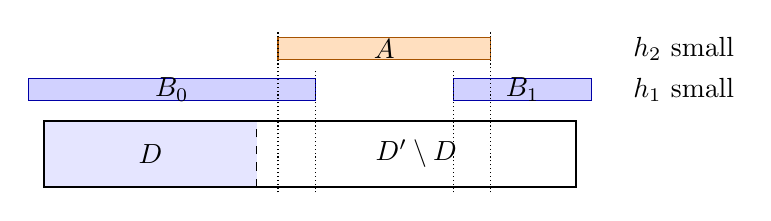
\begin{tikzpicture}[x=1.35cm,y=0.65cm]
 \fill[blue!10] (-2,-0.65) rectangle (0,0.65);
 \draw[thick] (-2,-0.65) rectangle (3,0.65);
 \draw[dashed] (0,-0.65)--(0,0.65);
 \node at (-1,0) {$D$};
 \node at (1.5,0) {$D'\setminus D$};
 \fill[blue!18] (-2.15,1.05) rectangle (0.55,1.48);
 \draw[blue!65!black] (-2.15,1.05) rectangle (0.55,1.48);
 \node at (-0.8,1.26) {$B_0$};
 \fill[blue!18] (1.85,1.05) rectangle (3.15,1.48);
 \draw[blue!65!black] (1.85,1.05) rectangle (3.15,1.48);
 \node at (2.5,1.26) {$B_1$};
 \fill[orange!25] (0.2,1.85) rectangle (2.2,2.28);
 \draw[orange!65!black] (0.2,1.85) rectangle (2.2,2.28);
 \node at (1.2,2.06) {$A$};
 \draw[densely dotted] (0.2,-0.75)--(0.2,2.4);
 \draw[densely dotted] (0.55,-0.75)--(0.55,1.65);
 \draw[densely dotted] (1.85,-0.75)--(1.85,1.65);
 \draw[densely dotted] (2.2,-0.75)--(2.2,2.4);
 \node[anchor=west] (first) at (3.45,1.26) {$h_1$ small};
 \node[anchor=west] (second) at (3.45,2.06) {$h_2$ small};
\end{tikzpicture}
\caption{Horizontal extents of the three compact pieces, shown in
separate rows. In the rectangular model, all three pieces share a vertical interval
slightly larger than that of $D'$. The two overlap bands control both
coordinates.}
\label{fig:pieces}
\end{figure}
